%% This is a skeleton file demonstrating the use of IEEEtran.cls (requires IEEEtran.cls version 1.8a or later) with an IEEE conference paper. 

%% 

%% Modified by Khan Reaz( kahn.reaz@ieee.org) 

%% Support sites: 

%% http://www.ieee.org/ 

  

%%*********************************************************** 

%% Legal Notice: 

%% This code is offered as-is without any warranty either expressed or implied; without even the implied warranty of MERCHANTABILITY or FITNESS FOR A PARTICULAR PURPOSE! 

%% User assumes all risk and can modify as s/he wants. 

  

%%*********************************************************** 

  

\def\b0{{\bf 0}} 

\def\ba{{\bf a}} 

\def\bb{{\bf b}} 

\def\bc{{\bf c}} 

\def\bd{{\bf d}} 

\def\be{{\bf e}} 

\def\bg{{\bf g}} 

\def\bh{{\bf h}} 

\def\bi{{\bf i}} 

\def\bj{{\bf j}} 

\def\bk{{\bf k}} 

\def\bl{{\bf l}} 

\def\bm{{\bf m}} 

\def\bn{{\bf n}} 

\def\bo{{\bf o}} 

\def\bp{{\bf p}} 

\def\bq{{\bf q}} 

\def\br{{\bf r}} 

\def\bs{{\bf s}} 

\def\bt{{\bf t}} 

\def\bu{{\bf u}} 

\def\bv{{\bf v}} 

\def\bw{{\bf w}} 

\def\bx{{\bf x}} 

\def\by{{\bf y}} 

\def\bz{{\bf z}} 

  

  

\def\bSigma{{\bf \Sigma}} 

\def\bA{{\bf A}} 

\def\bB{{\bf B}} 

\def\bC{{\bf C}} 

\def\bD{{\bf D}} 

\def\bE{{\bf E}} 

\def\bF{{\bf F}} 

\def\bG{{\bf G}} 

\def\bH{{\bf H}} 

\def\bI{{\bf I}} 

\def\bJ{{\bf J}} 

\def\bK{{\bf K}} 

\def\bL{{\bf L}} 

\def\bM{{\bf M}} 

\def\bN{{\bf N}} 

\def\bO{{\bf O}} 

\def\bP{{\bf P}} 

\def\bQ{{\bf Q}} 

\def\bR{{\bf R}} 

\def\bS{{\bf S}} 

\def\bT{{\bf T}} 

\def\bU{{\bf U}} 

\def\bV{{\bf V}} 

\def\bW{{\bf W}} 

\def\bX{{\bf X}} 

\def\bY{{\bf Y}} 

\def\bZ{{\bf Z}} 

  

  

%package list 

\documentclass[conference]{IEEEtran} 

\IEEEoverridecommandlockouts 

\let\labelindent\relax 

% \usepackage{breqn} 

\usepackage{enumitem} 

\usepackage{fleqn} 

\usepackage{cite} 

\usepackage{graphicx} 

\usepackage[varg]{newtxmath} 

\graphicspath{ {images/} } 

\usepackage{pdfpages} 

\usepackage{wrapfig} 

\usepackage{fancyhdr} 

\usepackage{lastpage} 

\usepackage{lettrine} 

\usepackage{amsmath} 

% \usepackage{titlesec} 

\usepackage{mathtools} 

\DeclarePairedDelimiter\ceil{\lceil}{\rceil} 

\DeclarePairedDelimiter\floor{\lfloor}{\rfloor} 

\usepackage[colorinlistoftodos]{todonotes} 

\usepackage{float} 

\usepackage[font={footnotesize}]{caption} 

\usepackage[numbers,sort,square,compress]{natbib} 

\usepackage[para]{footmisc} 

\usepackage{xcolor} 

\setlength{\belowcaptionskip}{-12pt} 

\newcommand{\highlight}[1]{% 

  \colorbox{red!50}{$\displaystyle#1$}} 

  

% \usepackage{parskip} 

% \setlength{\parskip}{0.02\baselineskip} 

  

% \fancypagestyle{plain}{ 

%   \fancyhf{} % sets both header and footer to nothing 

% \renewcommand{\headrulewidth}{0pt} 

%   \fancyhead[C]{2018 International Conference on Indoor Positioning and Indoor Navigation (IPIN), 24-27 September 2018, Nantes, France}% Right header 

  

% } 

\pagestyle{plain}% Set page style to plain. 

  

% \pagestyle{fancyplain} 

% \fancyhf{} 

% \renewcommand{\headrulewidth}{0pt} 

% \fancyhead[C]{2018 International Conference on Indoor Positioning and Indoor Navigation (IPIN), 24-27 September 2018, Nantes, France} 

\DeclareMathOperator*{\argmin}{argmin} 

% \usepackage{titlesec} 

  

% \titlespacing*{\section}{0pt}{1pt plus 2p}{1ex} 

% \titleformat*{\section}{\fontsize{12}{12}\bfseries} 

% \titleformat{\section} 

%        {\normalfont\fontfamily{phv}\fontsize{12}{17}\bfseries}{\thesection}{1em}{} 

  

% \titleformat{\subsection} 

%        {\normalfont\fontfamily{phv}\fontsize{12}{17}\bfseries\itshape}{\thesubsection}{1em}{} 

  

\begin{document} 

%Here goes the title 

  

\title{Scalar Parametrization for Joint Time-Frequency interpolation in a MIMO-OFDM channel} 

  

  

%Authors List 

  

\author{\authorblockN{Author 1, Author 2, Author 3} 

\ 

\authorblockA{Department of Electrical Engineering, Indian Institute of Technology Bombay} 

% \thanks{Parts of this work was supported by the Bharti Centre for Communication in 

% IIT Bombay, and the Visvesvaraya 

% PhD Scheme of Ministry of Electronics \& Information Technology, 

% Government of India (implemented by the Digital India Corporation). 

% }} 

} 

\maketitle 

  

\thispagestyle{plain} 

%Main body starts 

  

  

  

% \noindent We consider problem of quantization and interpolation of 

% time and frequency varying precoding matrices in wireless MIMO 

\begin{abstract} 

In a limited feedback MIMO channel, the performance of the channel can improve significantly if the transmitter knows the channel state information (CSI). The receiver knows the channel information, and it feeds back to the transmitter. However, it is not possible to feedback complete information for a limited-feedback OFDM channel since the channel information for multiple subcarriers consumes a large amount of data. Therefore, to resolve this problem, the orthonormality structure of the precoder matrix is exploited to make its one-to-one mapping to a minimal number of scalar parameters. The Precoder matrix is decomposed using Givens Rotation. For an i.i.d. flat-fading Rayleigh channel, these parameters are independent, which makes its quantization and interpolation easy. We propose an efficient method for quantization of the channel state information at the receiver by using adaptive delta modulation for successive time interval. We also propose a method for joint time-frequency interpolation of the channel information at the transmitter. 

\end{abstract} 

  

\section{Introduction} 
\label{intro}
% no need to write the numbers in your introduction. You start by explaining what is happening currently and then propose your solution. 

The use of multiple antennas at the transmitter and receiver can significantly enhance the performance of wireless systems. Moreover, in these multiple-input multiple-output (MIMO) wireless systems, the transmitter can perform better resource allocation if channel state information (CSI) is made available at the transmitter, both to improve data rates and reduce BER~\cite{love2008overview}. To this end, feeding back the CSI from the receiver to the transmitter efficiently is necessary. In wireless systems that use orthogonal frequency division multiplexing (OFDM), the feedback needs to be provided to the transmitter across all subcarriers, and this places a large feedback demand. However, since the CSI varies gradually in both time and frequency, effective techniques to reduce feedback overheads exist, using frequency domain interpolation temporal prediction. In particular, knowledge of the precoding matrices (that are typically the orthonormal right singular vectors of the channel matrix) is essential to achieve link capacity, as well as to parallelize the channel. In this paper, we focus on the problem of tracking the precoders of a MIMO-OFDM system across time and frequency for efficient CSI feedback. 
  
The problem of effective quantization and feedback of precoders for MIMO-OFDM has attracted significant attention in recent years. Many approaches involve codebook design over the Grassmann manifold~\cite{mondal2007quantization,schwarz2013adaptive,5946308} or the Stiefel Manifold \cite{6891198,Gupt1905:Predictive}, wherein the manifold structure of the precoders is used to obtain tangents for predictive quantization and interpolation across time and frequency. While these methods have been shown to be very effective for precoder feedback,  they involve operations over higher dimensional manifolds. In particular, optimization and interpolation is complicated, especially for manifolds where geodesic paths for interpolation may be difficult to obtain, especially for joint time-frequency predictive coding. An alternate approach is to parametrize the precoding matrices using scalar parameters. The space of unitary matrices parameterized into independent scalar parameters that correspond to Givens rotations and Household Transformations of the unitary precoding matrices \cite{4114278,4556174}. These approaches have been combined with adaptive delta modulation effectively track precoding matrices both in the time~\cite{4114278} and frequency domains~\cite{4556174}, albeit separately.

In this paper, we propose a method for exploiting the joint time-frequency correlation of the precoder's scalar parameters on the transmitter using CSI feedback. Typical approaches to predictive quantization and interpolation do not exploit the joint time-frequency correlation to enhance the precoder estimate at the transmitter. However, exploiting the correlations jointly not only reduces the feedback requirement, it also is able to enhance the precoder reconstruction accuracy. Further, the independence of the scalar parameters reduces the problem to interpolation of separate scalar valued function, as opposed to operations over tangent spaces in manifolds~\cite{Gupt1905:Predictive}. Simulations reveal that the proposed method offers matches the performance of manifold based approaches with a much lower implementation complexity and fewer number of bits.


The rest of this paper is organized as follows: Section~\ref{section2} described the system model and the precoder feedback and interpolation techniques. Section~\ref{section3} compares the BER and achievable rates for our proposed methods with that of past work. Finally, Section~\ref{section4} concludes with discussions on future work.

%Since $H=U\Sigma V$, it is sufficient to quantize V*(precoder) and send this information back. In an OFDM channel, this data consumes significant amount of bits and therefore, sending the complete data could consume too much bandwidth data. For e.g. an OFDM channel with 4 transmitters, 2 receiver antennas, and 64 subcarriers would require 64*(no. of bits required to send one precoder ~ 12-16 bits) ~ 896 bits per frame. This information could be significantly reduced if we provide better quantization and interpolation techniques/strategies. Also, the matrices which need to be fed back could be broken down into independent scalar parameters. These scalar quantities could be later quantized and interpolated. 

% Broad summary of your work, come to your problem definition. 

  

\section{System Model} 

\label{section2} 

For a MIMO-OFDM system with $N_T$ transmitter and $N_R$ receiver antennas, each subcarrier $i$ with time instant $t$ could be modelled as a flat-fading MIMO channel. This flat-fading MIMO channel could be modelled as 

\vspace{-1pt} 

\begin{equation} 
\by_{i,t} = \bH_{i,t} \bx_{i,t}+ \bf{\eta_{i,t}} 
\end{equation} 

\vspace{-1pt} 

where the channel matrix $\bH_{i,t} \in \mathbb{C}^{N_R \times N_T}$; the input $\bx_{i,t} \in \mathbb{C}^{N_T}$; the output $\by_{i,t} \in \mathbb{C}^{N_R}$ and $\eta$ is the complex additive white gaussian noise vector with distribution $\tilde{\mathcal{N}}(0,I_{N_R})$. On applying thin SVD to H, we get $\bH_{i,t} = U_{i,t} \Sigma_{i,t} V_{i,t}^{H}$, where $U_{i,t} \in \mathbb{C}^{N_R \times N_R}$, $\Sigma_{i,t} \in \mathbb{C}^{N_R \times N_R}$  and $V_{i,t} \in \mathbb{C}^{N_T \times N_R}$. $U_{i,t}$ and $V_{i,t}$ are orthonormal column matrices and $\Sigma_{i,t}$ contains the singular values $\sigma_1 \geq \ldots \geq \sigma_{N_T} > 0$ of H. The entries of H are assumed to be i.i.d. $\tilde{\mathcal{N}}(0,1)$, complex circularly symmetric Gaussian with mean zero and variance 1. Therefore, the first n column vectors of $V_{i,t}$ have to be quantized and fed back to the transmitter as channel spatial information.

% Givens rotation definition and how we are decomposing, Theta- pdf = 2lsin(theta)(2l-1).\cos(theta) 0 $\leq$ Theta $\leq$ pi/2. 
% Householders' transformation and how we are decomposing. -pi$\leq$ phi $\leq$ pi. Uniformly distributed. 
% Low-complexity quantization scheme based on a further parameterization of a vector in 
% terms of a minimal number of independent scalar parameters. In particular, we consider its application to CSI feedback in slowly time-varying MIMO channels 

\subsection{Scalar Parameterization} 
\label{givens}

The degrees of freedom in the spatial information matrix is much smaller than the number of real entries in the matrix because of the geometrical structure between the columns of the matrix \cite{4114278}. An orthonormal matrix with $t$ rows and $n$ columns can be represented as 

  

\begin{equation} 
\textbf{V} = \Bigg[\prod_{k=1}^{n} D_{k} \big( \phi_{k,k},\ldots , \phi_{k,n} \big) \: \Bigg\{ \prod_{l=1}^{l=t-k} G_{t-l,t-l+1} \big( \theta_{k,l}\big) \Bigg\} \Bigg] \: \tilde{I} 
\end{equation} 
  

where $D_{k}$ is the diagonal matrix given as $D_{k}\big(\phi_{k,k}, \ldots, \phi_{k,t} \big)$ =  $diag\big( 1_{k-1}, e^{j\phi_{k,k}},\ldots, e^{j\phi_{k,t}}  \big)$, $1_{k-1}$ is (k-1) ones; and t x n matrix $\tilde{I}$ = $\big[I_{n}, 0_{n,t-n}\big]^{T}$. The Givens matrix \textbf{G} is given as 

\begin{equation} 
G_{m-1,m}\big(\theta\big)  = 
\begin{bmatrix}

I_{m-2} & & & \\ 
& \cos\;\theta & - \sin\;\theta & \\ 
& \sin\;\theta & \cos\;\theta & \\ 
& & & I_{t-m}

\end{bmatrix} 
\end{equation} 
  

\begin{figure}
\label{adpm-fig}
\includegraphics[width=0.45\textwidth]{images/new-adpm-crop.pdf} 
\caption{Subcarriers which need to be quantized} 
\label{ber_overvie}
\vspace{-5pt} 
\end{figure} 


For a $4 \times 2$ orthogonal matrix V, 

$$V = D_{1}(\phi_{1,1},\ldots,\phi_{1,4}).G_{3,4}(\theta_{1,1}) .G_{2,3}(\theta_{1,2}) .G_{1,2}(\theta_{1,3})$$ 

\vspace{-1.4em} 

\hspace{1pt}$$.D_{2}(\phi_{2,2},\phi_{2,3},\phi_{2,4}) .G_{3,4}(\theta_{2,1}) .G_{2,3}(\theta_{2,2}).\tilde{I}$$ 

  

Here, we denote $\phi_{i}'s$ by phases and $\theta_{i}'s$ by rotation angles. $\phi \in (-\pi, + \pi]$ is uniformaly distributed between the two extremes\cite{4114278}, while $\theta$ has a distribution 

\begin{equation} 
p(\theta) = 2l\sin(\theta)^{2l-1}\cos(\theta), \theta \in [0, \frac{\pi}{2}), for \; l = 1,2,\ldots,t-1
\end{equation}

Here all $\theta_i$ and $\phi_i$ are statistically independent which is usefel for tracking them across time as explained in the next subsection. The total number of parameters obtained from the decomposition of a complex orthogonal matrix $N_{T} \times N_{R} $ is given by the relation $N_{R}(2N_{T} - N_{R}) $ \cite{4114278}. Number of $\phi = N_{R}(2N_{T} - N_{R}-1)/2$ while the number of $\theta = N_{T}(2N_{T} - N_{R}+1)/2$ 

% may cross pi and come immediately to -pi, therefore, values are unwrapped while calculating them. Unwrapping is performed at the receiver over the frequency initially and later in time. 

% To exploit the interpolation of time \& frequency jointly at the transmitter, feedback bits are sent in an alternating fashion as shown in the figure. 

  

\subsection{Differential Quantization - Channel Tracking} 
\label{quantiz} 

For a slowly time varying channel, ADPM is an effective method for tracking a paramater over time with using only 1-bit. The 1-bit number $\beta_{n} = Q(x_{n} - \hat{x}_{n-1})$ where $x$ is the unquantized vector $\&$ $\hat{x}$ is the quantized vector and $Q(x)$ is the quantization function given as 

  

\begin{equation}
  Q(x)=\begin{cases}
    1, & \text{if $x>0$}.\\
    -1, & \text{otherwise}.
  \end{cases}
\end{equation}

Thus, the quantied vector $\hat{x}_n$ changes with time as 

\begin{equation} 
\hat{x}_{n} = \hat{x}_{n-1} + \beta_{n}\Delta_{n} 
\end{equation} 

\begin{equation}
\label{delta_eqn}
\Delta_{n} = \begin{cases} 
    M \Delta_{n-1}, & \text{if $\beta_{n} = \beta_{n-1}$}.\\ 
    \Delta_{n-1}/m , & \text{if $\beta_{n} \neq \beta_{n-1}$}. 
  \end{cases} 
\end{equation} 

Here we initialize delta using $\Delta_1 = abs(x_{2}-\hat{x}_1)$.

We need to quantize the subcarriers in a way such that we can exploit the joint time-frequency interpolation at the transmitter side. Therefore, we select the subcarriers for quantization in an alternating fashion as shown in the figure. Figure shows a \textbf{N} subcarrier MIMO channel with subcarriers which are going to be quantized at the position sk, k = 0,1,...,$\frac{N-1}{s}$ for even time instance. Here, s is the gap between two frequencies. For odd time instances, subcarriers at the position sk + t for k = 0,1,..., $\frac{N-1}{s}$ with t = $\floor*{\frac{s}{2}}$. 

Therefore, in ADPCM channel tracking scheme, the arrows in the figure show how previous quantized values along with the 1-bit number find the new quantized value. Now with the above discussion, the bit budget for each subcarrier will be equal to number of scalars * 1-bit. On an average, this can be reduced to half if we transmit only $\theta$ values for one-time instance and only $\phi$ values for the next time while keeping the un transmitted values same as the previous one. This was, the average number of bits required to quantize a channel matrix will be $N_{T}(2N_{T} - N_{R})/2$. 

One problem associated with the tracking of phases ($\phi$) is that they change abruptly (cite the figure) between $-\pi$ and $\pi$ since $\sin/\cos(\pi) =\sin/\cos(-\pi)$. Therefore we have to wrap around the values by removing those abrupt changes (/cite another figure here). 

% We initialize $\hat{x}$ i.e. $\hat{x}_1$ by quantizing the $x_1$ using $\textbf{B}$ bits. 

\subsection{Joint Time Frequency Interpolation} 
\label{interp} 

After obtaining the $\beta$ values(1-bit numbers) at the trasnmitter we will calculate the subcarrier indices at indices sk or sk+t. To reproduce the rest of the subcarriers will use future time instances to do the interpolation. As you can see in the figure, each parameter is interpolated using the subcarriers of the next six time instances. We do the interpolation using the spline-cubic interpolation. We could also use other standard techniques by calculating the MMSE at the missing subcarrier locations but the spline-cubic interpolation method gives better results over the other method. 

Now here we can see the advantage of using subcarriers in an alternating fashion as given in the previous section. With this method we could exploit both time and frequency correlation because 

%Explain prediction and quantization steps here itself ! (succintly) 

\section{SIMULATION AND DISCUSSION} 
\label{section3}

 We have performed simulations to analyse the performance of the proposed quantization and interpolation method for slowly time-varying MIMO OFDM channel. Channel is simulated using the typical Jakes Model for both ITU Vehicular-A channel and ITU Pedestrian Channel. Performance is measured by averaging over 10 channel realizations with 100 simulations each. The normalised doppler frequency $f_{norm} = f_{max}.T_s$ is set to $3.5\times10^{-4}$ with sampling frequency $T_s = 20MHz$. For both vehicular and pedestrian channel, $N_T=4$ and $N_R=2$. Therefore, the total number of parameters are $N_{R}(2N_{T} - N_{R}) = 12$ with 5$\theta$’s and 7$\phi$’s. There are 1024 subcarriers in Vehicular channel and 64 subcarriers in the Pedestrian Channel. We take s = 33/9 for Vehicular and pedestrian channel respectively I.e. 32/8 equally spaced subcarriers with indices 33t/9t, t = 0,1, … , 31 and 0,1, .. ,7 respectively.  

\subsection{Initial Quantization} 
For the first and the second simulations/time instances we use of $\textbf{B}$ = 10 bits for quantizing each parameter for effective quantization/initialization. Therefore, the number of bits for each subcarrier = $10\times12$ = 120. Quantization is performed as given in Section~\ref{section2}. 

Simulation: BER is calculated by averaging over all the simulations. For Vehicular Channel, 1024 subcarriers are used with doppler frequency – and sampling rate = $10^{5}$

Initialization is performed by using $10\times12$ bits for each subcarrier for the initial two time frames. Later, the quantization will take place in the time-domain using one bit for each parameter. Since the bit budget is low and we are considering slowly varying channels, therefore, either theta or phi parameters are sent alternatingly in the time domain while keeping the unsent parameters equal to their previous values as show in the Figure \ref{adpm-fig}. Here $\Theta$ is the the collection of all $\theta$'s and $\Phi$ is the collection of all $phi$'s. This brings down the bit budget to average of 5(Size of $\Theta$) and 7(Size of $\Phi$) i.e. 6 bits average per fed back subcarrier. 

\bf{ADPM Design}: The decrement rate - \bm is 2.4 times the \bM - increment rate in the Equation~\ref{delta_eqn} . This ratio was decided after trying with different ratios. This implies that if quantied values loose track of the actual values then after changing delta quickly they start following it again.
Also, need to describe the initialization of the Delta values required in the quantization process. Need to cite that paper. We should also try over different quantization rates to compare 

While doing interpolation at the transmitter end, future time instances are used to interpolate the rest of the subcarriers indices which are not fed back. To prevent much delay, we are using 6 future time instances and using SciPy cubic interpolation over each parameter in 2D. These interpolated values and then used to reconstruct the precoding matrices all together. 

Performance Measurements: 
Since the Precoding matrices fundamentally lie on the Stiefel manifold, therefore, we are using the chordal distance parameter to measure the effectiveness of the quantization method used by us. Later we are comparing the BER rates with the ideal completely fed back subcarriers. 

Using the idea of joint interpolation given in the other paper. 

%talk about this in the simulations, that would be more relevant 
Since $\Delta_{n} = M\Delta_{n-1} or \Delta_{n-1}/m $, we found empirically that $m=2.4*M$ i.e. decay 

\begin{figure} 
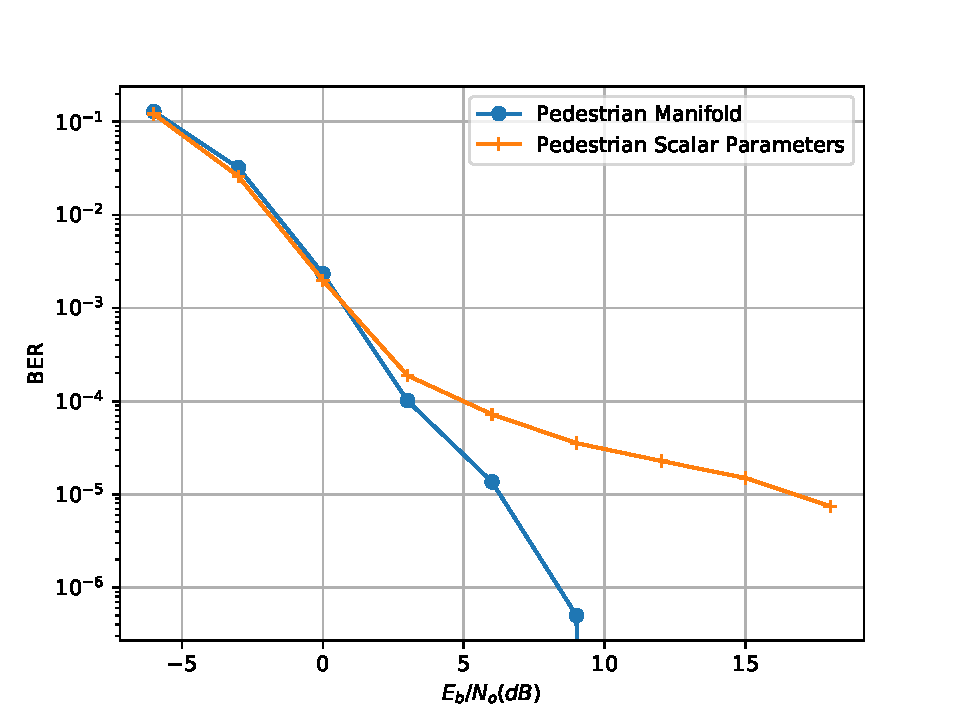
\includegraphics[width=0.5\textwidth]{images/pedestrian.pdf} 
\caption{BER vs SNR for pedestrian channel} 
\label{ber_overview} 
\vspace{-5pt} 
\end{figure}

\subsection{Performance Measurement} 

\label{setting} 

  

\noindent Since the Precoding matrices fundamentally lie on the Stiefel manifold, therefore, we are using the chordal distance parameter to measure the effectiveness of the quantization method used. Later we are comparing the BER rates with the completely fed back subcarriers. Or simulations and discussions part 2 criteria could be used. Done similar work as in \cite{4114278} but along with that we have joint interpolated in time and frequency at the transmitter using the fundamental scalar parameters obtained. To lower the number of bits we have used the method of interpolation and have achieved significant improvement over predictive quantization method in \cite{6891198} and also in \cite{Gupt1905:Predictive} which tried to use joint interpolation over the tangent space in the Stiefel Manifold. In fact, we use joint interpolation of the scalar parameters which are easy to use and give better quantization than any of the above methods.

The advantage they had over the number of bits due to the 6 bit codebook in \cite{6891198,Gupt1905:Predictive} is also achieved by us by using smart interpolation techniques, i.e. by dropping the feedback bits in alternating time instances as it is still going to follow the scalar parameters without much difference.

The problem of values hopping between $\pi$ and $-\pi$ is also tackled by wrapping the values around which we can show works nicely. The only drawback is that while initializing the parameter, they go out of their actual range and therefore using a uniform quantizer over the prescribed range does not work. But since most of the values lie between the given range we can use most of the initialization bits quantizing the parameters uniformly between the [-$\pi$ , $\pi$] and using smaller amount of bits between the range outside that which could go up to $-3\pi$ and $3\pi$, i.e. we are covering 300% more range outside the given area and that works mostly fine for the rest of the values. 

Using the idea of joint interpolation given in the other paper. 

\begin{figure} 
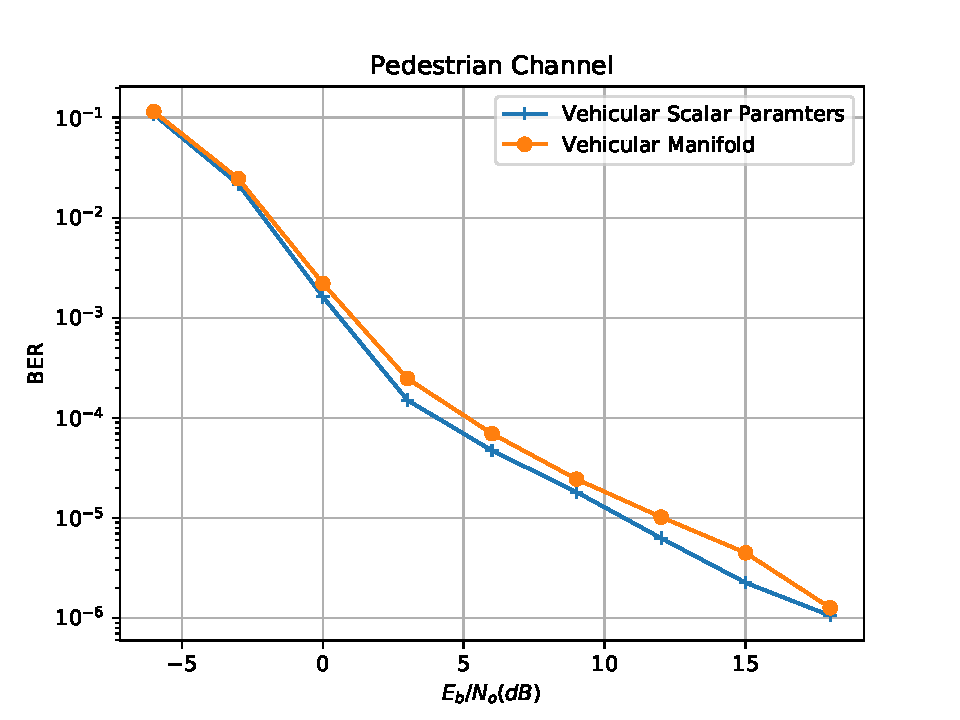
\includegraphics[width=0.5\textwidth]{images/vehicular_ber.pdf}
\caption{BER vehicular plot comparison between our method and \cite{Gupt1905:Predictive}} 
\label{ber_overview} 
\vspace{-5pt} 
\end{figure} 
%Qtisn error with 1000 chan evols 
%Qtisn error with 100 chan evols 
%BER 
%Achievable rat 
\section{Conclusions and Future Work} 
\label{section4} 

We could reduce more by seeing the effect of sigma values (power distribution). We can save the bits by not sending for those which have very low sigma values. This could result in a very robust method. 

\vspace{-4pt} 

  

% \section{Acknowledgment} 

% % \label {section6} 

% % \input{sections/6_section.tex} 

% Parts of this work was supported by the Bharti Centre for Communication in 

% IIT Bombay, and the Visvesvaraya 

% PhD Scheme of Ministry of Electronics \& Information Technology, 

% Government of India, being implemented by Digital India Corporation. 

  

  

\renewcommand{\bibfont}{\footnotesize} 

\bibliography{IEEEabrv,main} 

\bibliographystyle{IEEEtran} 

\end{document} 
